\chapter{Marco contextual}
Los sistemas de información han sido de gran utilidad en estos últimos años, obteniendo ciertos beneficios como automatizar el manejo de los datos, generación automática de reportes y desarrollar sus actividades de forma más eficiente y productiva. Cada organización cuenta con algún sistema de información de acuerdo a sus necesidades y actividades.

No obstante, existe ciertos problemas dentro de un sistema de información, ya sea por su grado de dificultad, problemas de diseño, consistencia e integridad de los datos almacenados.

\section{Ingeniería de software}
\cite{sommerville2005ingenieria} define a la ingeniería de software como una disciplina de ingeniería que se interesa por todos los aspectos de la producción de software, desde las primeras etapas de la especificación de sistema hasta el mantenimiento del mismo después de que se pone en operación. \cite{sommerville2005ingenieria} destaca dos frases clave:

\begin{enumerate}
\item \textbf{Disciplina de ingeniería:} Los ingenieros aplican técnicas y métodos de ingeniería para hacer que las cosas funciones, aun cuando no existen teorías y métodos aplicables, además de trabajar bajo ciertas restricciones organizacionales y económicas.
\item \textbf{Todos los aspectos de la producción de software:} La ingeniería de software no solo incluye los procesos de desarrollo de software, si no que también comprende la administración del proyecto de software y el uso de herramientas y teorías que puedan ser de utilidad en la producción de software.
\end{enumerate}

El enfoque sistemático que comúnmente se usa en la ingeniería de software se conoce comúnmente como proceso de software. Un proceso de software es una secuencia de actividades que conducen a la elaboración de un producto de software. \citep{sommerville2005ingenieria} menciona cuatro actividades fundamentales de este proceso:

\begin{enumerate}
\item \textbf{Especificación del software:} Los clientes y los programadores llegan a un acuerdo sobre qué software se producirá y bajo qué restricciones.
\item \textbf{Desarrollo del software:} Se diseña y programa el software.
\item \textbf{Validación del software:} Se verifica si es lo que acord´desarrollar y que funcione correctamente.
\item \textbf{Evolución del software:} Se modifica el software para ajustarse a los requerimientos del cliente y del mercado.
\end{enumerate}

\section{Programación Extrema (eXtreme Programming)}

\subsection{Agilidád}
Para comprender de una mejor manera este concepto, es necesario conocer el concepto de \emph{agilidad} en el ámbito de la ingeniería en software. \cite{jacobson2000lenguaje} tiene la siguiente definición:

\begin{displayquote}
Un equipo ágil es diestro y capaz de responder de manera apropiada a los cambios. El cambio es de lo que trata el software en gran medida. Hay cambios en el software que se construye, en los miembros del equipo, debidos a las nuevas tecnologías, de todas clases y que tienen un efecto en el producto que se elabora o en el proyecto que lo crea. Deben introducirse apoyos para el cambio en todo lo que se haga en el software; en ocasiones se hace porque es el alma y corazón de éste. Un equipo ágil reconoce que el software es desarrollado por individuos que trabajan en equipo, y que su capacidad, su habilidad para colaborar, es el fundamento para el éxito del proyecto.
\end{displayquote}

Esto nos dice que el ingeniero de software debe de ir rápido si quiere ir adaptándose a los cambios. La agilidad también incluye actitudes y estructuras de equipo que hacen más fácil la comunicación entre los ingenieros y los gerentes.

La agilidad puede aplicarse casi para cualquier proceso de software, para lograr esto se tiene que diseñar de tal forma que se le permita al equipo adaptar las tareas y desarrollarlas con fluidez, concentrarse en los productos de trabajo esenciales y hacer énfasis en una estrategia de entrega incremental que haga trabajar al software tan rápido como sea posible para el cliente, según el tipo de producto y el ambiente de operación.

\subsection{Programación Extrema}
La Programación Extrema (XP) es una metodología ágil definida por Kent Beck. Según \cite{canos2012metodologias} ésta metodología está centrada en potenciar las relaciones interpersonales como clave para el éxito en desarrollo de software, promoviendo el trabajo en equipo, preocupándose por el aprendizaje de los desarrolladores, y propiciando un buen clima de trabajo. XP se basa en la retroalimentación continua entre el cliente y el equipo de desarrollo, comunicación fluida entre todos los participantes, simplicidad en las soluciones implementadas y coraje para enfrentar los cambios. XP se define como especialmente adecuada para proyectos con requisitos imprecisos y muy cambiantes, y donde existe un alto riesgo técnico.

\subsection{Proceso XP}

\begin{itemize}
\item \textbf{Planeación:} Esta actividad comienza escuchando a los demás integrantes del equipo con el fin de recabar los requerimientos de software. Esto conlleva a la creación de \emph{historias de usuario} que describen las salidas, caracterizaras y funciones del software, el cliente les asigna un valor o prioridad. Posteriormente es analizada por los demás integrantes del equipo y se le asigna un costo medido en semanas de desarrollo.
\item \textbf{Diseño:}
\item \textbf{Codificación:}
\item \textbf{Pruebas:}
\end{itemize}

\begin{figure}[H]
	\begin{center}
		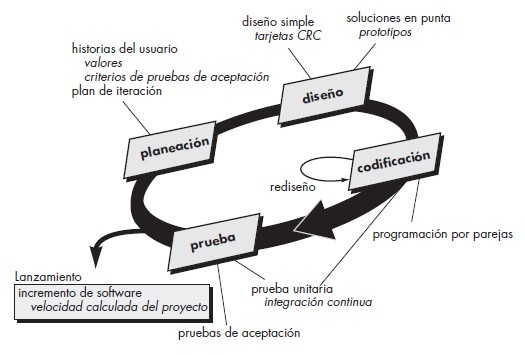
\includegraphics{imagenes/procesoxp.jpg}
		\caption{Proceso de la Programación Extrema (\cite{pressman2005ingenieria}).}
		\label{pxp}
	\end{center}
\end{figure}

\subsection{Historias de usuario}
Es una técnica utilizada para la determinación de los requisitos de software. Son tarjetas de papel, en donde el cliente describe de forma breve y clara las características que el software debe contener, ya sean requisitos funcionales o no funcionales en un lenguaje no técnico (\cite{canos2012metodologias}).

\begin{table}[H]\small
\caption{Ejemplo de una historia de usuario.}
\label{ehu1}
\begin{tabular}{@{\extracolsep{\fill}} | p{2.5cm} | p{2.5cm} | p{2.5cm} | }
\multicolumn{3}{|c|}{\textbf{1.} Aplicación didáctica} \\ \hline
  \hline
\multicolumn{3}{|p{15cm}|}{Como usuario quiero que la aplicación sea didáctica y de aprendizaje mediante ejercicios.} \\ \hline
\hline
\textbf{Estimación:} 7 semanas &	\textbf{Valor:} 50	& \textbf{Dependencias:} \\
\hline
\multicolumn{3}{|p{15cm}|}{\textbf{Condiciones de satisfacción:}
\begin{itemize}
	\item La aplicación contendrá información selecta y bien explicada.
	\item Se incluirán algunos ejercicios los cuales deberán resolverse en la computadora.
\end{itemize}
}\\ \hline
\hline
\end{tabular}
\end{table}

La esctructura de una historia de usuario consiste en los siguientes elementos:

\begin{itemize}
\item \textbf{Número de historia:} El numero que corresponde a la historia.
\item \textbf{Nombre de la historia:} Debe ser breve y claro.
\item \textbf{Descripción:} Es una explicación breve en lenguaje no técnico de la función que va a realizar el sistema.
\item \textbf{Estimación:} El tiempo que llevará desarrollar dicha función.
\item \textbf{Valor:} El numero de importancia que se le asigna a la historia.
\item \textbf{Dependencias:} Indica la historias de usuario que dependen de esta misma.
\item \textbf{Condiciones de satisfacción:} Son restricciones bajo las cuales se desarrollará la historia de usuario.
\end{itemize}

\subsection{Roles en XP}
Los roles que \cite{beck1999embracing} propone son:

\begin{itemize}
\item \textbf{Programador:} Es el encargado de producir el código del sistema y llevar a cabo las pruebas unitarias.
\item \textbf{Cliente:} Es el que escribe las historias de usuario y los requerimientos funcionales para su implementación, asigna la prioridad a las historias de usuario y decide cuales se implementaran en cada iteracion.
\item \textbf{Encargado de pruebas (\emph{tester}):} Es el encargado de ejecutar las pruebas y ayuda al cliente a escribir las pruebas funcionales.
\item \textbf{Encargado de seguimiento:} Es quien verifica el grado de acierto en las estimaciones realizadas con el tiempo real que se utilizó, dando seguimiento para mejorar futuras estimaciones.
\item \textbf{Entrenador (\emph{coach}):} Es el responsable de todo e proceso, guiando al equipo con el fin de que se aplique el proceso de XP de forma correcta y eficiente.
\item \textbf{Consultor:} Es un miembro externo al equipo con un conocimiento de un tema en especifico en el que pueda surgir algún problema.
\item \textbf{Gestor (\emph{Big boss}):} Es el enlace entre el cliente y los programadores, coordinando al equipo a que trabajen con las condiciones adecuadas de forma efectiva.
\end{itemize}

\section{Lenguaje de Modelado Unificado (UML)}

El Lenguaje de Modelado Unificado (UML por sus siglas en inglés) es un lenguaje de modelado no un proceso o un método. UML está compuesto por una notación muy especificas y reglas semánticas relacionadas para la construcción de un sistema de software. UML tiene un amplio conjunto de elementos de notación gráfica. Estos pueden ser clases, componentes, nodos, actividades, flujos de trabajo, casos de uso, objetos y estados. Además de como relacionar estos elementos entre si (\cite{sparks2000introduccion}).

\section{Notación}
\subsection{Vistas}
Las vistas muestran los diferentes aspectos del sistema que está siendo modelado. No es un gráfico, sino una abstracción que consiste en una serie de diagramas. Cada vista mostrará aspectos particulares del sistema, dando enfoque a ciertos ángulos y niveles, y con esto podría ser construida una imagen completa del sistema (\cite{burgues2014aprende}).

\subsection{Modelos}
Los modelos representan una abstracción de una entidad en la que se esté trabajando (\cite{burgues2014aprende}).

\section{Elementos estructurales}
Éstos son elementos estáticos y representan comúnmente cosas conceptuales o materiales. \cite{alarcon2000diseno} describe los siguientes.

\subsection{Clases}
Una clase es una descripción de un conjunto de objetos que comparten los mismos atributos, relaciones, operaciones y semántica. Una clase puede implementar una o mas interfaces. Está representada como un rectángulo con sus nombre, atributos y operaciones.

\begin{figure}[H]
	\begin{center}
		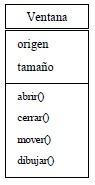
\includegraphics{imagenes/clase.jpg}
		\caption{Representación gráfica de una clase.}
		\label{clase}
	\end{center}
\end{figure}

\subsection{Interfaz}
Es una colección de operaciones que especifican un servicio de una determinada clase o componente. Una interfaz describe el comportamiento de varias operaciones pero nunca su implementación. La interfaz solo muestra los componentes visibles externos o solo una parte. Está representada por un circulo.

\begin{figure}[H]
	\begin{center}
		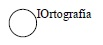
\includegraphics{imagenes/interfaz.jpg}
		\caption{Representación gráfica de una interfaz.}
		\label{interfaz}
	\end{center}
\end{figure}

\subsection{Colaboración}
Una colaboración define una interacción y es un conjunto de roles y otros elementos que colaboran para proporcionar un comportamiento cooperativo mayor que la suma de los comportamientos de sus elementos. Las colaboraciones tiene una dimensiones tanto estructural, como de comportamiento. Está representado por una elipse con borde discontinuo.

\begin{figure}[H]
	\begin{center}
		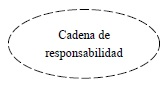
\includegraphics{imagenes/colaboracion.jpg}
		\caption{Representación gráfica de una colaboracion.}
		\label{colaboracion}
	\end{center}
\end{figure}

\subsection{Casos de uso}
Un caso de uso es la descripción de un conjunto de acciones que un sistema ejecuta y produce un determinado resultado que es de interés para un actor en general. Se usa principalmente para organizar el comportamiento de un modelo. Está representado por una elipse con borde continuo.

\begin{figure}[H]
	\begin{center}
		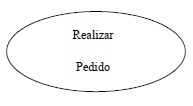
\includegraphics{imagenes/caso-de-uso.jpg}
		\caption{Representación gráfica de un caso de uso.}
		\label{cuso}
	\end{center}
\end{figure}

\subsection{Actor}
Un actor es una persona, sistema o despositivo que interactua con el sistema, iniciando, recibiendo resultados o participando en un caso de uso (\cite{gil2003representacion}). Se representa de la siguiente manera:

\begin{figure}[H]
	\begin{center}
		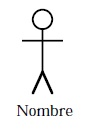
\includegraphics{imagenes/actor.jpg}
		\caption{Representación gráfica de un actor.}
		\label{actor}
	\end{center}
\end{figure}

\subsection{Clase activa}
Es una clase cuyos objetos tienen uno o mas hilos en ejecución y por lo tanto pueden dar lugar a actividades de control. Se representa de la misma forma que una clase, pero con bordes mas gruesos.

\begin{figure}[H]
	\begin{center}
		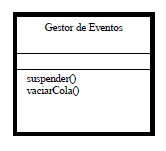
\includegraphics{imagenes/clase-activa.jpg}
		\caption{Representación gráfica de una clase activa.}
		\label{claseactiva}
	\end{center}
\end{figure}

\subsection{Componentes}
Un componente es una parte física y reemplazable de un sistema que proporciona interfaces y la implementación de dicho conjunto. Un componente representa comúnmente el empaquetamiento físico de diferentes elementos lógicos, como clases, interfaces y colaboraciones.

\begin{figure}[H]
	\begin{center}
		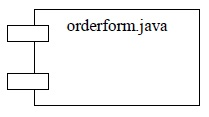
\includegraphics{imagenes/componente.jpg}
		\caption{Representación gráfica de un componente.}
		\label{componente}
	\end{center}
\end{figure}

\subsection{Nodos}
Es un elemento físico que existe en el tiempo de ejecución. Representa un recurso computacionál que dispone algo de memoria, y con frecuencia, de capacidad de procesamiento.

\begin{figure}[H]
	\begin{center}
		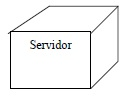
\includegraphics{imagenes/nodo.jpg}
		\caption{Representación gráfica de un nodo.}
		\label{nodo}
	\end{center}
\end{figure}

\section{Elementos de comportamiento}
Estos elementos son las partes dinámicas del modelo, y representan el comportamiento del tiempo y el espacio.

\subsection{Interacción}
Este comportamiento comprende una serie de mensajes intercambiados entre un conjunto de objetos, dentro de un contexto en particular para llegar a un resultado en específico. Puede involucrar muchos otros elementos, como mensajes secuencias de acción y enlaces.

\begin{figure}[H]
	\begin{center}
		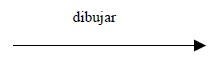
\includegraphics{imagenes/interaccion.jpg}
		\caption{Representación gráfica de una interacción.}
		\label{interaccion}
	\end{center}
\end{figure}

\subsection{Máquinas de estado}
Es un comportamiento que especifica los distintos estados por los que v pasando un objeto o las interacciones durante su vida en respuesta a eventos. Una máquina de estado puede involucrar a muchos otros elementos, como estados transiciones, eventos y actividades.

\begin{figure}[H]
	\begin{center}
		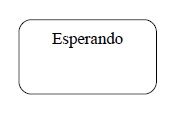
\includegraphics{imagenes/maquina-de-estado.jpg}
		\caption{Representación gráfica de una maquina de estado.}
		\label{maquina}
	\end{center}
\end{figure}

\section{Elementos de agrupación}
El principal elemento de agrupación es el paquete, cuyo propósito es organizar los distintos elementos en grupos. Un paquete es solamente conceptual (existe solamente en el tiempo de desarrollo). Gráficamente se representa como una carpeta con su nombre, y a veces, su contenido.

\begin{figure}[H]
	\begin{center}
		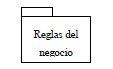
\includegraphics{imagenes/paquete.jpg}
		\caption{Representación gráfica de un paquete.}
		\label{paquete}
	\end{center}
\end{figure}

\section{Elementos de anotación}
Estos elementos son partes explicativas de los modelos UML. Son comentarios que se usan para describir, clasificar y hacer observaciones sobre cualquier elemento de un modelo.

\begin{figure}[H]
	\begin{center}
		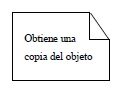
\includegraphics{imagenes/nota.jpg}
		\caption{Representación gráfica de una nota.}
		\label{nota}
	\end{center}
\end{figure}

\section{Relaciones}
En las relaciones se habla de una clase destino y de una clase origen. La clase origen es desde la que se realiza la acción de relacionar. Es decir, desde la que parte la flecha. La clase destino es la que recibe la flecha. Las relaciones se pueden modificar con estereotipos o con restricciones.

\subsection{Dependencia}
Es una relación semántica entre dos elementos en el cual, un cambio a un elemento (el elemento independiente) puede afectar a la semántica del otro (elemento dependiente). Se representa por una linea discontinua, posiblemente dirigida, y que puede incluir una etiqueta.

\begin{figure}[H]
	\begin{center}
		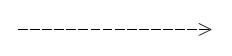
\includegraphics{imagenes/dependencia.jpg}
		\caption{Representación gráfica de una relación de dependencia.}
		\label{dependencia}
	\end{center}
\end{figure}

\subsection{Asociación}
Es una relación estructural que describe un conjunto de enlaces, los cuales son conexiones entre objetos. La agregación es u tipo de relación y representa una relación estructural entre un todo y sus partes. La asociación se representa con un alinea continua, posiblemente dirigida y que a veces incluye una etiqueta.

\begin{figure}[H]
	\begin{center}
		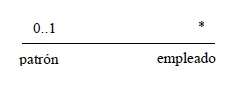
\includegraphics{imagenes/asociacion.jpg}
		\caption{Representación gráfica de una relación de asociación.}
		\label{asociacion}
	\end{center}
\end{figure}

\subsection{Generalización}
Es una relación de generalización/especialización, en la cual los objetos del elemento especializado (el hijo) pueden a los objetos del elemento general (el padre). De esta forma, el hijo comparte la estructura y comportamiento del padre. Se representa con una linea con una punta de flecha vacía.

\begin{figure}[H]
	\begin{center}
		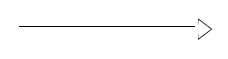
\includegraphics{imagenes/generalizacion.jpg}
		\caption{Representación gráfica de una relación de generalización.}
		\label{generalizacion}
	\end{center}
\end{figure}

\subsection{Realización}
Es una relación semántica entre clasificadores, donde un clasificador especifica un contrato que otro clasificador garantiza que cumplirá. Se pueden encontrar relaciones de realización en dos sitios: entre interfaces y las clases y componentes que las realizan, y entre los casos de uso y las colaboraciones que los realizan. Se representa con una linea discontinua con una punta de flecha vacía.

\begin{figure}[H]
	\begin{center}
		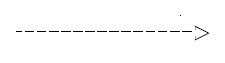
\includegraphics{imagenes/realizacion.jpg}
		\caption{Representación gráfica de una relación de realización.}
		\label{realizacion}
	\end{center}
\end{figure}

\section{Diagramas}
En UML existen distintos diagramas que muestran el comportamiento o la estructura de un sistema, mostrando distintas perspectivas del mismo.

\subsection{Diagrama de clases}
Este diagrama muestra un conjunto de clases, interfaces y colaboraciones, así como sus relaciones. Cubren la vista de diseño estática.

\subsection{Diagrama de secuencia y colaboración}
Los diagramas de secuencia y los de colaboración son diagramas de interacción. Consisten en un conjunto de objetos y relaciones, incluyendo los mensajes que puedan tener de un objeto a otro. La diferencia entre ambos diagramas es que el diagrama de secuencia enfatiza el ordenamiento temporal de los mensajes, mientras que en los diagramas de colaboración se muestra la estructura de los objetos que envían mensajes.

\subsection{Diagrama de casos de uso}


\subsection{Diagrama de estructura}

\section{Sistema de información}
Para comprender de una mejor manera este concepto, primero abordaremos los conceptos de \emph{sistema} e \emph{infomación}.

\subsection{Sistema}

\subsection{Información}

\

\section{Modelo Entidad-Relación}
